% sec_experiments.tex — simulation study (R3/R5 data)
\section{Simulation Study}\label{sec:experiments}

This section reports the simulation campaign. Its evidential status is stated
precisely at the outset: the campaign is an \emph{implementation-level
consistency check}---it verifies that the platform computes what the theorems
predict (truth mode: exact tensor enumeration; sample mode: trajectory
estimation validated against truth) and that no registered falsification
window is violated---together with mechanism demonstrations that carry
information beyond the proofs (the blind zone's parameter-domain capture, the
defense-direction monotonicity, and the BB-2 calibration of what violating
the black-box certified bound's premise costs). It is not an external-validity
study: one tabular substrate, no independent platform, no human subjects
(Section~\ref{sec:limitations}); zero refutations is the \emph{expected}
outcome of a correctly implemented consistency check, not independent
evidence for the theory; and the scenario names below (\emph{prompt
injection}, \emph{filter bubble}, \emph{learned helplessness},
\emph{sycophancy}) are \emph{toy analogues} for the corresponding surgery
classes on a substrate with no language, no retrieval, no pretraining, and no
multi-step planning---no empirical test of the named real-world phenomena.
The design principle: a criterion is a falsification window operationalized;
verdicts are \textsc{confirmed}/\textsc{refuted}/\textsc{inconclusive}, a
\textsc{refuted} verdict may not be edited away by changing criteria, and
defense compression pushing an arm out of its registered window is recorded
\textsc{inconclusive} (out of window), never counted as refutation. All
verdicts are computed in truth mode unless explicitly marked (the sample mode
is exercised and validated separately, \S\ref{sec:estimators}); the 360
\textsc{inconclusive} runs are registered with their (scenario,
configuration, seed) coordinates in the archived run manifest.

\subsection{Platform and protocol}

The benchmark platform ENV-0 is a tabular substrate: a ring resource grid
($E=(x,u)$, position and supply level), five actions
$\Acal=\{\text{left},\text{right},\text{harvest},\text{idle},\text{exit}\}$, a
resource clock $Z$, and noisy observation of position buckets. The agent
architecture instantiates the framework's wiring: internal state
$S=(G,B,M,R)$ (goal grid index $G$ as the endorsement object; belief buckets
$B$; self-model and register buckets $M,R$), a softmax policy over one-step
expected utility, and a grid-quantized contractive endorsement map.
Interventions compile to the loci of \eqref{eq:factorization} ($\beta_G$
goal planting, $\beta_\pi$ policy-script switching, $\gamma$
observation-kernel replacement, $\delta$ action-set contraction, $\alpha$
honest information, $\sigma^{\pm}$ resource-kernel modification).

Two compute modes are used: a \emph{truth mode} (exact tensor enumeration of
the joint law) and a \emph{sample mode} (trajectory simulation). Full causal
logs $(E,O,S,A,Z,I)$ per step are mandatory and schema-validated---by
Proposition~\ref{prop:unidentifiable}, without them $\Lam$ is in principle
unidentifiable, so the logging requirement is an identifiability necessity.
Seeds derive deterministically from (scenario, configuration, replication)
coordinates (formula: Appendix~\ref{app:counting}), so every run is
bit-reproducible.

\subsection{Scenario library and matrix}

Fifteen scenarios implement the falsification windows:
\textbf{ATK-1} reward hijacking/shaping ($\beta_G$ gradient, sweeping
strength $\eta$; T3a, T5-goal, AX3/$\Lam$, $\AHI$); \textbf{ATK-2} filter
bubble/retrieval poisoning ($\gamma$; T3a/b, T4 both sides, T2 blindness
witness, T1d sub-threshold arm, script corollary); \textbf{ATK-3} dependency
injection/lock-in ($\delta$+time; C1, C2, T5-exec, EWS); \textbf{ATK-4} prompt
injection reaching behavior ($\alpha$ masquerading as $\beta$; T2 attribution,
four-track observabilization); \textbf{ATK-5} urgency manipulation
($\tau$-compression; T5-ref, T6 gate monotonicity); \textbf{ATK-6}
sub-threshold slow drift ($\beta$; \textbf{T6 key experiment}: design rule,
$\Amin$ per-run check, blind zone, $\deltastar$ ablation, registration domain,
detection divergence); plus independent groups \textbf{DEL-1} (delegation
$(\lambda,q)$ grid plus direct-flow and $\rho\neq1$ bracket arms; T7),
\textbf{C0-DEMO} (injection vs verbatim principal
instruction; Proposition~\ref{prop:c0}), \textbf{LH-1} (helplessness
induction; human-side counterpart), \textbf{RES-1} (resource starvation
$\sigma^-$; T5-via, T1b converse), \textbf{$\sigma^-$-EROSION} (capability
envelope erosion; extended T5-via gate, D-via), \textbf{FORCE-1} (forced
autonomy; T8),
\textbf{BB-1} (black-box degradation; \S\ref{sec:identifiability}),
\textbf{C0-CORR} (projection consistency; Proposition~\ref{prop:c0}(i)), and
\textbf{EXEC-1} (rich-coupling arm restoring $\Aexec$ dynamic range;
T5-exec).

The main matrix is ATK-1--6 $\times$ $8$ defense configurations
($2^3$: registration M1 / endorsement gate M2 / redundancy M4, each on or off)
$\times$ $\varsigma\in\{0.5,1\}$ $\times$ 30 seeds $=6\times8\times2\times30
=2{,}880$ runs;
a $\varsigma=2$ arm ($1{,}440$ runs) is an axiom-relaxation
stress test (AX5 relaxed), reported separately and on the same footing as the
$\varsigma<1$ checks (Corollary~\ref{cor:sigma-band}); independent groups add
$300$ runs ($7\times30=210$ across the seven independent scenarios
(DEL-1, C0-DEMO, C0-CORR, LH-1, RES-1, FORCE-1, BB-1)
plus the $30$-run adaptive-adversary supplement BB-2 and the $60$-run
supplement of this revision ($\sigma^-$-EROSION and EXEC-1,
below). Campaign total: $2{,}880+1{,}440+300=4{,}620$ runs in approximately
$32$ minutes on a commodity workstation (8-core CPU, 32\,GB RAM).

\paragraph{Counting units (two bundle registries, stated apart).}
A \emph{run} is one (scenario, defense configuration, $\varsigma$, seed)
execution; a \emph{cell} is the 30-run block at fixed (scenario, defense,
$\varsigma$); a \emph{bundle} is a registered six-component record
($\Aorg,\Agoal,\Aexec,\Aepi,\Aref,\Avia$) within a run's metrics. Because
different analyses pool bundles differently, the two pools are registered
apart---with the full per-scenario composition, the defense-direction count,
and the seed-derivation formula in Appendix~\ref{app:counting}:
(i) \emph{arm bundles} (the row-level attack-strength records of ATK-1/2/4,
the only per-strength-bundle scenarios): $5{,}760$ main-matrix $+2{,}880$
stress $=8{,}640$---the weight-sensitivity pool; (ii) the \emph{recursive
registry} (every embedded six-component record, arm bundles plus non-row
records): $7{,}290$ over the main matrix and EXEC-1---the T1a range
meta-criterion pool---and $11{,}250$ across the full campaign (the X3
alternative-aggregation pool); the exact $7{,}290-5{,}760=1{,}530$
difference is decomposed in the appendix. A \emph{criterion
count} ($N$ in Table~\ref{tab:main}) is per-falsification-window verdicts.
Run-level verdicts:
$2{,}520$ \textsc{confirmed} $+360$ \textsc{inconclusive} $=2{,}880$.

\paragraph{Registered effect sizes (SESOI).}
Sign-based criteria carry a registered smallest effect size of interest:
composite-level strict-decrease criteria (T3a family) require a drop of at
least $0.01$ in $A$ (an order of magnitude above the truth-mode numerical
floor and comparable to the largest sample-mode estimator error, $0.0096$,
\S\ref{sec:estimators}); blindness witnesses require the blind channel's
change below $10^{-3}$ while a covering channel's response exceeds $10^{-3}$;
the T7 linear-law tolerance is $5\%$; ratio criteria are reported with
$95\%$ seed CIs. Criteria are thus not bare sign tests; effect sizes are
reported with the verdicts in the archived report.

\subsection{Main results}\label{sec:exp-results}

\begin{table}[htbp]
\centering
\caption{Main results: proposition-level verdicts over the full campaign
(fifteen criteria; the detection-impossibility control of
Proposition~\ref{prop:detection} is exercised as a carrier arm of T6,
ATK-6(vi)). The column conventions and the run-level totals are stated in
the reading guide immediately following the table.}
\label{tab:main}
\footnotesize
\setlength{\tabcolsep}{4pt}
\begin{tabularx}{\textwidth}{@{}l l
>{\raggedright\arraybackslash}X
>{\raggedright\arraybackslash}X
>{\raggedright\arraybackslash}X@{}}
\toprule
Proposition & Type / evidence & Content & Carrier & Verdict ($N$) \\
\midrule
T1a & definitional / replay & range $0\le A\le1$ & matrix range scan + witness tests & \textbf{CONFIRMED} ($7{,}290$ registry bundles---pool (ii) of Appendix~\ref{app:counting}---$0$ violations) \\
T1b & definitional / replay & operational positivity & RES-1 & \textbf{CONFIRMED} (60/60) \\
T1c & definitional / replay & conditional strict upper bound & baseline bundles & \textbf{CONFIRMED} ($A\in[0.079,0.374]$) \\
T1d & bound / replay & undetectable manipulation exists & ATK-2(v) & \textbf{CONFIRMED} (60/60) \\
T2 & architectural / replay & attribution + multi-channel necessity & ATK-4, ATK-2(ii) & \textbf{CONFIRMED} (240/240) \\
T3a & substantive / replay & manipulation $\Rightarrow$ $A$ strictly decreases (layered; L0/L1 $\beta_G$-on-$\Fix$ corner registered) & ATK-1(iii), ATK-2(i), FORCE-1 & \textbf{CONFIRMED} (180/180) \\
T3b & bound / replay & covert $\Rightarrow$ $\mathbb{E}[\Aphen]\ge\mathbb{E}[A]-\varepsilon$; expected gap monotone & ATK-2(iii)(iv) & \textbf{CONFIRMED} (120/120; expectation-level bound with Markov firing floor, not a pointwise inequality) \\
T4 & optimization / replay & highest-leverage attack, water-filling defense ($\varsigma=1$) & ATK-2(vi)(vii) & \textbf{CONFIRMED} (120/120) \\
T5 & definitional / replay & six-disjunct loss & ATK-1(ii), ATK-3(v), ATK-4(ii), ATK-5(iii), RES-1, $\sigma^-$-EROSION & \textbf{CONFIRMED} (330/330) \\
T6 & substantive / replay; seeded (vi) & autonomy margin & ATK-6(i)--(vi), ATK-5(ii) & \textbf{CONFIRMED} (420/420) \\
T7 & substantive / replay (algebra) & delegation laws & DEL-1(i)--(vi) & \textbf{CONFIRMED} (180/180) \\
T8 & definitional / replay & coercion consistency & FORCE-1(i)--(iii) & \textbf{CONFIRMED} (90/90) \\
C0 & construction / construction; seeded TV & behaviorally identical, autonomy separable & C0-DEMO, C0-CORR & \textbf{CONFIRMED} (150/150) \\
C1 & toy / algebra (n=1) & fold transition, critical slowing & ATK-3(i)(ii) & \textbf{CONFIRMED} (120/120) \\
C2 & toy / algebra (n=1) & open hysteresis loop & ATK-3(iii) & \textbf{CONFIRMED} (60/60) \\
\bottomrule
\end{tabularx}
\end{table}

\paragraph{How to read Table~\ref{tab:main}.} ``Type'' records the claim's
evidential grade: \emph{substantive}, \emph{architectural} (premise-conditional
consistency of the measurement wiring), \emph{optimization},
\emph{definitional-layer}, \emph{bound}, \emph{construction}, or \emph{toy}
(phase-line properties of a chosen normal form). ``Evidence'' records the
verdict's class, not the theorem's: \emph{replay} = deterministic truth-mode
evaluation (no statistical content, effectively $n=1$); \emph{seeded} =
sampled statistic with a $95\%$ CI; \emph{construction}; \emph{algebra} =
deterministic integration of the stated normal form. C1/C2 are algebra checks:
their run counts are replications of the same integration, not independent
evidence. ``Carrier'' lists the scenarios implementing each window; $N$ =
criterion-level confirmations. Run level: $2{,}520$ CONFIRMED, $360$
INCONCLUSIVE (the defense-arm runs outside their window, by construction),
\textbf{$0$ REFUTED}.

Table~\ref{tab:main} gives the proposition-level verdicts.
The evidential asymmetry is marked in the display itself, because it is the
most common misreading of this table: rows whose evidence class is
\emph{replay}, \emph{construction}, or \emph{algebra} are implementation
consistency checks---their verdicts would obtain under any correct
re-implementation, so the ``$15/15$'' headline is a statement about the
discipline of the registry (no window violated), not fifteen independent
empirical confirmations of the theory. The rows that carry information beyond
the proofs are the seeded statistics and the mechanism demonstrations
(blind-zone capture, $\sigma^-$-EROSION gate witness, EXEC-1 dynamic-range
restoration, BB-2 premise calibration); none of them touches the
external-validity question, which remains the registered decisive next
experiment (Section~\ref{sec:threats}(xi)). The quantitative anchors:

\paragraph{Statistical reporting.}
Two disjoint classes of numbers are reported, and they are not mixed.
\emph{Deterministic replays}: criteria evaluated on truth mode over
deterministic dynamics (the C1/C2 scalings, the T7 linear law, the
blind-zone boundaries) are exact computations---their $R^2=1.0000$ and
zero-width slope intervals are properties of deterministic evaluation, carry
no statistical content, and are reported without interval interpretation
(effectively $n=1$ as evidence; their role is numerical verification of the
algebra). \emph{Seeded statistics}: wherever a statistic depends on sampling
(the estimator two-path validation, the OU-noise early-warning series, the
C0 sampled-TV check, the detection-divergence ratio), we report $95\%$
confidence intervals with $n=30$ seeds; proportions of the form $30/30$ carry
the binomial 95\% lower confidence bound $\approx0.884$ (Clopper--Pearson,
two-sided) and are strong but not certain. The fifteen criteria are
structural verdicts over exact computations, not a family of hypothesis
tests, so no multiplicity correction applies to them; where seeded statistics
feed a criterion (the BB-1/BB-2 bound checks), the CIs are the report. A
further consequence deserves explicit statement: for the deterministic
classes, ``more seeds'' cannot change a verdict---the replications establish
bit-reproducibility, not statistical power---and the $n=30$ design with
reported CIs and the Clopper--Pearson floor is the power statement exactly
where the evidence is genuinely sample-based (the estimator two-path
validation, the OU early-warning series, the C0 sampled-TV check).

\begin{table}[htbp]
\centering\small
\caption{Quantitative anchors of the campaign, collected for independent
recomputation. ``Deterministic'' marks exact truth-mode computations (no
statistical content); ``seeded'' marks $n=30$ sampling with $95\%$ intervals;
the Clopper--Pearson entry is the two-sided 95\% lower confidence bound of
any $30/30$ proportion.}
\label{tab:anchors}
\footnotesize
\begin{tabularx}{\textwidth}{@{}>{\raggedright\arraybackslash}X l
>{\raggedright\arraybackslash}X l@{}}
\toprule
Anchor & Value & Reference point & Class \\
\midrule
mediation witness $I(I;A)=1-H_b(0.1)$ & $0.531$~bit & $\Fext=0$ under the
same law (direction reversal) & deterministic \\
$30/30$ proportions & CP lower bound $0.884$ & --- & seeded \\
detection-divergence ratio & $1.951\pm0.034$ & theory $\to2$
(Lorden--Lai asymptotic, Prop.~\ref{prop:detection}) & seeded \\
C1 recovery scaling slope & $-0.504\pm0.000$, $R^2=1.0000$ & theory $-0.5$
& deterministic \\
EXEC-1 dynamic-range restoration & $0.234/0.017=13.7\times$ & exact chain
$0.234>0.218>0$ & deterministic \\
T7 linear-law maximal deviation & $2.0\times10^{-5}$ & registered tolerance
$5\%$ & deterministic \\
X5-a endorsement-quantization continuum limit &
$\Agoal^\infty(\eta)=1-2\eta/(1+\eta)$ & stationary gap
$\eta(1-\eta)^2/(2(1+\eta))$, max $0.0567\le0.057$ & deterministic \\
X5-b $\kappa$-layer attenuation & $1/|\kappa|$ & $0.500\to0.250$ as
$|\kappa|:2\to4$ (deep-capture floor) & deterministic \\
blind-zone capture / design-rule boundedness & $30/30$ both directions &
Corollary~\ref{cor:blindzone} & deterministic (seeded count) \\
\bottomrule
\end{tabularx}
\end{table}

\begin{itemize}
\item \textbf{T6 (key experiment)}. Design rule ($\theta/W\le\kappa\Rightarrow$
globally bounded damage $<0.99$) and $\Amin$ per-run check: all runs.
Blind-zone prediction (Corollary~\ref{cor:blindzone};
Figure~\ref{fig:blindzone}): under $\theta/W>\kappa$
with $\delta\in(\kappa,\theta/W)$, zero registrations fire and $D\to1$
on the mismatched channel \emph{despite} the full mechanism stack being
present---30/30 replications, both directions (Clopper--Pearson 95\% lower
bound $0.884$).
$\deltastar$ ablation reproduces the exact $\min$-term structure (disabling
M1/M3/M4 collapses $\deltastar$ to the corresponding remaining minimum; all
disabled $\Rightarrow$ $\deltastar=0$). The detection-divergence control arm
replicates Proposition~\ref{prop:detection}: halving $\delta$ multiplies
damage at detection by $1.951\pm0.034$ (30 seeds).
\item \textbf{C1/C2}. The recovery-time scaling fits
$\Trec\propto(\delta_c-\delta)^{-1/2}$ with slope $-0.504\pm0.000$
(theory $-0.5$) and $R^2=1.0000$ over 30 seeds; the hysteresis loop stays open
with independently positive thresholds $\delta_{down}=0.0701$,
$s_c=0.2347$; the three early-warning indicators ($\Trec$, stationary
variance, AR(1)) are all monotone approaching criticality.
\item \textbf{T7}. Under equal-strength calibration (H1', including the
$\Fext^{self}=0$ premise, which the platform satisfies \emph{by
construction}---so the exact fit below verifies the implementation of the
bookkeeping, and is \emph{not} independent validation of the law), the
linear law
$\Aorg=\Aorg^{self}(1-\lambda(1-q))$ holds (Figure~\ref{fig:t7}) with maximal
deviation $2.0\times10^{-5}$ over the measured grid
(exact to $10^{-9}$ at the five equal-strength calibration strengths;
registered tolerance 5\%); the composite identity is exact ($<10^{-9}$) with the
weight-regression slope $w_{org}$ significant and positive; the $q=1$ arm has
$\Fext\equiv0$ ($<10^{-12}$), confirming the $\alpha$-equivalence.
Two further arms exercise the bracket
(Proposition~\ref{prop:bracket}) where H1$'$ fails: a \emph{direct-flow
arm} ($f>0$, i.i.d.\ flag switching), where the measured direct flow
($0.671/0.844/0.799$ nats at $m=0.3/0.5/0.7$) leaves the realized $\Aorg$
($0.0030/0.0017/0.0011$) strictly below the linear-law prediction
($0.70/0.50/0.30$)---content bookkeeping understates delegation flow by two
orders of magnitude here, $C_{self}$ being tiny---while the
$\varphi$-relaxed two-sided bracket ($\rho\in[0.9,1.1]$,
$\varphi\le T\ln2/\Fint^{self}$) contains the realized value in all arms;
and a \emph{$\rho\neq1$ arm} ($C_{del}=1.5\,C_{self}$), where the bracket
with $\rho\in[1.35,1.65]$ contains the realized $\Aorg$ while the linear
law breaches its 5\% tolerance---the bracket is the right object off the
calibrated locus.
\item \textbf{T5-via extension ($\sigma^-$-EROSION; D-via)}. The extended
gate \eqref{eq:avia}---$\Avia$ the minimum of the resource ratios and the
capability margins $m_j$---is exercised across an erosion grid
$\kappa_{eff}=(1-\varepsilon)\kappa_0$,
$\varepsilon\in\{0,0.4,\ldots,1.0\}$: the margin region
($\varepsilon\le0.5$) leaves $\Avia=1$, the binding region degrades
monotonically ($0.8,0.6,0.4,0.2$), full erosion gives
$\Avia=A=0$ on both tracks, and a repair-budget-collapse arm ($R_{eff}=0$,
$\kappa$ intact) gives the same---witnessing the $\min$-factor structure;
the $m=1$ regression anchor reproduces the resource-only gate value $0.835$
pointwise in the non-vacuous domain. Crucially, all five channel components
and $\Lam$ are pointwise invariant across the erosion arms
($\le10^{-12}$): pure $\sigma^-$ capability erosion is \emph{invisible to
every channel monitor} and caught only by the gate (Figure~\ref{fig:p3gate}(a)).
\item \textbf{EXEC-1 ($\Aexec$ dynamic range)}. On the compact v1 instance
the execution channel reads $\Aexec=0.017$ (the pinned-near-zero caveat of
the scale-anchoring paragraph below); the rich-coupling arm (fine-grained
position observation, $|\mathcal{O}|=4$, observation noise $0.05$) lifts it
to $0.234$ ($13.7\times$), and the $\delta$-contraction chain replicates
exactly down to the zero-empowerment helplessness signature of
Proposition~\ref{prop:wd-exec} ($0.234>0.218>0$; composite $0.647>0.637>0$;
Figure~\ref{fig:p3gate}(b)).
\item \textbf{C0}. The two arms (principal's verbatim instruction vs covert
injection) are behaviorally identical (sampled TV $=0.0000\pm0.0000$; truth
marginals pointwise equal at $10^{-12}$), while $\Aepi^{real}$ ($0.5$ vs $1$,
accuracy against the logged ground truth)
and $\Lam$ ($0$ vs $1$ law-level---the covert $\gamma$ is in the surgery
history at full strength) separate them; projection consistency across 12
configurations has
Kendall $\tau=1.000$ on matched dimensions with projection-direction checks
passing.
\item \textbf{T2 multi-channel necessity (matrix-level)}. Aggregating the
per-arm component bundles, the blind-witness table reads: $\beta_G$ is
detected by $\{\Agoal,\Aref\}$, $\gamma$ by $\{\Aepi,\Aexec,\Aref\}$,
$\beta_\pi$ by $\{\Aorg,\Aref\}$ (the $\Aref$ response is
$\Lam$-mediated via \eqref{eq:lambda}, so external scripts are visible at
law level even when behavior is instructive), urgency manipulation ($\tau$)
by $\{\Aref\}$, and $\delta$ lock-in by $\{\Aexec\}$ (EXEC-1 arms). No
single component covers all surgery classes---and every component is blind to
at least one class---over all $7{,}290$ registered bundles, with zero range
violations and zero ``death without attribution'' (every $A<10^{-6}$ bundle
has a zeroed disjunct).
\item \textbf{Hallucination index (T3b, $\S$\ref{sec:dualtrack};
Figure~\ref{fig:ahi})}. Under
covert $\beta_G$/$\gamma$ arms, $\AHI>0$ appears while the corresponding
component has degraded but not collapsed (the early-warning register), and
the gap
$\Aphen-\Aobj$ grows monotonically with attack strength; ATK-1(iv) and
ATK-2(iii)(iv) confirmed over all cells. \emph{Pooling labels} (the two
quotations are kept distinct on purpose): the headline series
$0\to0.110\to0.204\to0.374$ is the \emph{undefended cell at
$\varsigma=1$} (also the configuration-wise maximum and the $95\%$ band's
upper edge); Figure~\ref{fig:ahi} displays \emph{medians over all (defense
configuration, $\varsigma$, replication) cells}
($0\to0.057\to0.092\to0.126$)---defense suppression is exactly what the
median measures, so the two series differ by construction, not by error.
\item \textbf{Defense direction}. Across the $8$ defense configurations,
defended arms at equal nominal attack strength show never-more damage
($840/840$ matched comparisons across ATK-1/2 combined---$420$ per
class---the two classes with implemented coupling rules; coupling for
ATK-3--6 is a placeholder, registered in \S\ref{sec:limitations}).
\end{itemize}

\paragraph{Scale anchoring (the benign baseline).}
The unperturbed baseline composite lies in $A\in[0.079,0.374]$ (T1c)---a
consequence of the non-degeneracy conditions, not a calibration accident:
T1c's D1--D4 (observation noise, incomplete self-model, residual or
constrained resources) hold in any physically finite agent and each pulls $A$
strictly below $1$; $A=1$ is the ideal limit AX1 excludes. The operational
anchor for deployments is therefore the calibration-period percentile band of
$A$ over registered benign operation, not the value $1$: ``normal'' is the
band, ``fully autonomous'' is the limit.
Two channel-level anchors are reported for transparency, since they bound the
composite's dynamic range. (i) \emph{Execution}: the ENV-0 empowerment
normalizer is $n\log|\Acal|=\log 5\approx1.609$ nats, while the realized
$\Aexec^{obs}\approx0.010$ under the passive protocol---the channel's
reachable band is narrow on the default instance, so
$\Aexec^{w_{exec}}$ acts as a nearly constant suppression factor on the
composite there; the percentile-band reading above is the operational
response. The EXEC-1 arm of this revision re-instantiates the channel with
real dynamic range (finer observation, lower noise): $\Aexec$ lifts to
$0.234$ and the $\delta$-contraction chain replicates exactly down to the
zero-empowerment signature, so the narrow band is a property of the default
instance's coupling, not of the component definition
(\S\ref{sec:limitations}(x)). (ii) \emph{Goal}:
the ENV-0 endorsement map has contraction modulus $c=0.5$ and the
maximally-alienated scale $\dc=2.0$ (grid units), with the baseline goal
sitting exactly at the endorsed fixed point---$\Agoal=1.000$ at baseline is a
statement about the fixed point's location, not a degenerate reading; the
$0/0$ fallback of \eqref{eq:agoal} is not triggered anywhere in the campaign.
(iii) \emph{Epistemic}: the baseline accuracy is
$\Aepi=0.811$ under observation noise $0.15$---the strict inequality
$\Aepi<1$ at baseline is the D1 clause of T1c made quantitative, and the
ATK-2 grid gives the degradation profile $0.811\to0.718\to0.625\to0.500$
across $s(\gamma)\in\{0,0.3,0.6,1.0\}$.

\begin{figure}[t]
\centering
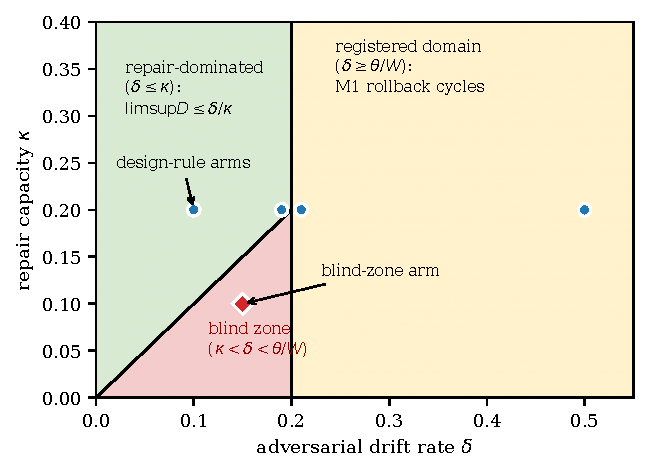
\includegraphics[width=.55\textwidth]{figures/fig_t6_blindzone.pdf}
\caption{T6 margin geometry at $\theta/W=0.2$ (ATK-6 constants): the
repair-dominated region ($\delta\le\kappa$), the blind zone
($\kappa<\delta<\theta/W$), and the registered domain ($\delta\ge\theta/W$).
Markers: the four design-rule arms (blue; bounded 30/30) and the blind-zone
arm (red; captured 30/30 with the full mechanism stack present).}
\label{fig:blindzone}
\end{figure}

\begin{figure}[t]
\centering
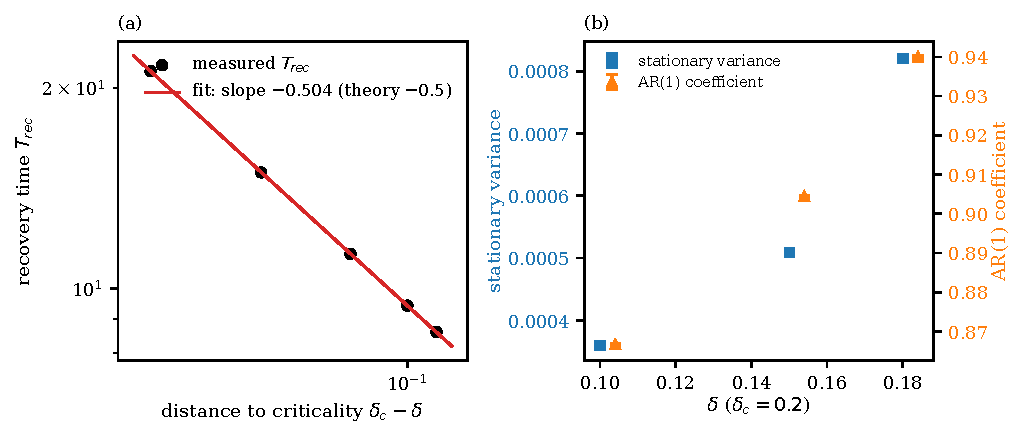
\includegraphics[width=\textwidth]{figures/fig_ews_c1.pdf}
\caption{C1 critical slowing in ATK-3. (a) Recovery time vs.\ distance to
criticality, log--log: measured points and the fitted power law
(slope $-0.504$, theory $-0.5$; $R^2=1$ because the dynamics are integrated
deterministically). (b) The OU-noise early-warning indicators across the
$\delta$ grid: stationary variance (blue, tolerance-registered) and AR(1)
coefficient (orange) rise toward criticality with $95\%$ CIs over 30 seeds.}
\label{fig:ews}
\end{figure}

\subsection{Robustness: axiom-relaxation checks in the elasticity parameter}
\label{sec:sigma}

Per Corollary~\ref{cor:sigma-band}, the full axiom set admits $\varsigma=1$
only; the bands around it are \emph{relaxation} checks, reported as such. All
conclusions are recomputed across $\varsigma\in[0.5,1]$: zero verdict flips
between the $\varsigma=0.5$ and $\varsigma=1$ arms (the elasticity-flip
meta-check). T4 is the one criterion whose \emph{content} changes with
$\varsigma$, and its two verdicts are reported separately: the vertex
(concentration) verdict holds at $\varsigma=1$, and the pre-registered
interior-KKT signature (no vertex concentration) is what the
$\varsigma\neq1$ arms confirm---the same label covers two different,
pre-registered predictions, and the table entry is the $\varsigma=1$ one.
The $\varsigma=2$ stress arm
(AX5 relaxed) flips no verdict either, but exhibits the predicted quantitative
signature: at the complete-capture arm of ATK-1, $A$ is exactly $0$
for $\varsigma\le1$ (zero annihilation) but $0.1652>0$ at
$\varsigma=2$---the
scenario-level echo of the axiom's failure, which is why
$\varsigma>1$ is
excluded from the framework and retained only as a stress test.

\subsection{Supplementary analyses}\label{sec:supplement}

Three analyses, run \emph{post hoc} over the campaign's registered component
bundles (components are $\varsigma$- and weight-independent truth values;
only the composite is recomputed), strengthen the robustness claims; X5 of
\S\ref{sec:e2checks} adds two architecture-level re-runs (the
construct-validity arms).

\paragraph{Weight sensitivity (protocol obligation of
Section~\ref{sec:representation}).}
All campaign composites were recomputed under five alternative weight
vectors (channel-heavy and extreme variants, e.g.\ $w_{goal}=0.45$) over the
$8{,}640$ campaign arm bundles (pool (i) of Appendix~\ref{app:counting}):
zero range violations;
zero-annihilation preserved exactly ($120/120$ complete-capture arms stay
$0$); T3a monotonicity unbroken ($0/960$ cells); ordering against equal
weights stable (Kendall $\tau\in[0.930,1.000]$ over the $5{,}760$ main arms,
the minimum attained by the
deliberately extreme vector). The T4 attack point moves \emph{by
construction} ($\arg\max_i w_is_i/c_i$ depends on $w$): under equal weights
the epistemic channel is the optimal target in $480/480$ cells, and under an
origination-heavy vector the optimum splits between origination and epistemic
($240/480$ each)---the comparative static, not a defect. A caveat travels with
every weight and channel-count conclusion below: on the default ENV-0 instance
the execution channel reads $\Aexec^{obs}\approx0.010$, so the composite is
effectively four-channel-plus-suppression there
(Section~\ref{sec:limitations}(x)); the weight analysis probes ordering
stability, not the full five-channel dynamic range---which the EXEC-1 arm
verifies is recoverable by richer coupling rather than absent by definition.
\emph{Weight and elasticity sensitivity, rerun on the rich-coupling
instance} (closing the evidence gap just named; components are truth values,
so the recomputation is exact---artifact
\texttt{analysis\_exec1\_weights.json}): over the EXEC-1
$\delta$-contraction chain (rich $0.234$ $>$ movement-preserving $0.218$ $>$
non-movement-preserving $0$ in $\Aexec$), recomposing under all five
alternative weight vectors preserves the verdict chain
$0.647\!>\!0.637\!>\!0$ (composite \emph{levels} shift, $0.570$--$0.742$
for the rich arm, while the zero-empowerment arm stays exactly $0$ by
annihilation---one chain point is pinned at zero, so the ordering check is
necessary-but-coarse, reported as such); the elasticity band
$\varsigma\in\{0.25,0.5,0.75,1\}$ preserves the chain, and
$\varsigma=2$ exhibits the expected annihilation failure ($A=0.545$, vs.\
$0.1652$ on the compact matrix). With the fifth channel at full dynamic
range, the same weight battery flips no verdict.

\paragraph{Extended elasticity band.}
Recomposing every arm at $\varsigma\in\{0.25,0.5,0.75,1\}$: zero range
violations, zero T3a violations, and exact zero at the complete-capture arm
for every $\varsigma\le1$ (the $\varsigma=2$ stress arm remains the lone
AX5-violating echo at $A=0.1652$). Per the status stated at the head of
Section~\ref{sec:sigma}, these arms are robustness evidence under axiom
relaxation, not validity claims for $\varsigma<1$ (which violates
\textup{(A6)}).

\begin{figure}[t]
\centering
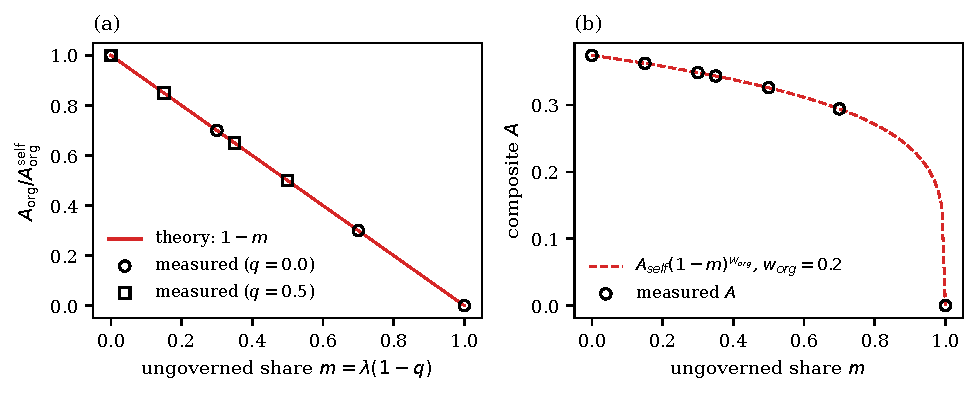
\includegraphics[width=\textwidth]{figures/fig_t7_delegation.pdf}
\caption{T7 delegation laws (DEL-1). (a) Component linear law
$\Aorg/\Aorg^{self}=1-m$ with $m=\lambda(1-q)$: measured points at
$q\in\{0,0.5\}$, maximal deviation $2.0\times10^{-5}$ under the (H1')
calibration. The platform satisfies (H1$'$) by construction, so the fit is an
implementation check of the bookkeeping, not empirical validation of the
law. (b) Composite law $A=A_{self}(1-m)^{w_{org}}$: measured
composite against the fitted curve.}
\label{fig:t7}
\end{figure}

\begin{figure}[t]
\centering
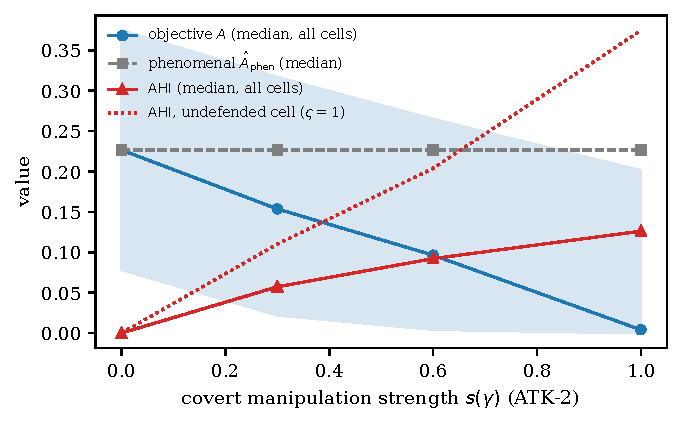
\includegraphics[width=.6\textwidth]{figures/fig_ahi.pdf}
\caption{T3b hallucination index (ATK-2 covert $\gamma$ arms). Solid curves
and bands: medians with $5$--$95\%$ bands pooled over all (defense
configuration, $\varsigma$, replication) cells; the dotted curve is the
undefended cell at $\varsigma=1$ (all defenses off), whose AHI series
$0\to0.110\to0.204\to0.374$ is the headline quotation in the text---the
pooled median series reads $0\to0.057\to0.092\to0.126$, the difference being
defense suppression, not a discrepancy. Note that the median AHI is not the
difference of the two displayed median curves (medians do not commute with
subtraction): at $s=1$ the visible gap between the median curves exceeds the
median AHI because defended cells suppress $\Aobj$ and $\AHI$ jointly.
The AHI is a one-sided alarm by design---elevation flags covert
self-overestimation; silence is never evidence of absence---and the minimal
two-sided extension is registered, not run
(Section~\ref{sec:threats}(viii)).}
\label{fig:ahi}
\end{figure}

\paragraph{Adaptive adversaries and the black-box bound (BB-2): a
sensitivity calibration.}
The $\Aorg$ rule of Section~\ref{sec:blackbox} is certified for
bypass-semantics exogenous probes, and only the upper end is certified.
BB-2 (30 runs) calibrates what the premise violation costs: an
adversary whose injection timing conditions on the agent's state
($G=\theta^*$; per-state flags compiled through the same $\beta_\pi$
machinery) violates the bypass premise $I^t\ind S^t\given A^{t-1}$ of the
randomized-probe route. Control arms (iid flags,
state-independent script): zero violations of the certified upper bound
($2/2$; and the reference band happens to enclose the truth---a heuristic
observation, not a containment claim). Adaptive arms at
$p\in\{0.3,0.5,0.8\}$: the certified bound's bypass premise is violated in
$3/3$ arms; the naive exogenous plug-in then \emph{overestimates} the
external flow (bias $+0.17$, $+0.39$, $+0.90$ nats, truth-mode exact) and
the bound no longer holds---e.g.\ at $p=0.5$, truth $\Aorg=0.33$ against an
upper end of $0.006$ computed under the violated premise (where the premise
fails, the certificate is void, not refuted). The bias figures are deterministic
exact computations (identical across seeds), so the $3/3$ is not a
small-sample failure: premise violation \emph{deterministically} voids the
certificate in these arms, and the calibration's content is the size of the
inflation, not a frequency. The demonstration is thus a sensitivity
calibration rather than a confirmation: adaptive timing is enough to inflate
the plug-in by $+0.17$--$+0.90$ nats, so the
bypass premise is practically fragile even though the rule is formally
correct within its scope. Auditing adaptive adversaries requires causal-layer
access---the estimation-side counterpart of
Corollary~\ref{cor:logs-necessary}.

\paragraph{Controls and ablations.}
The campaign contains three negative-control constructs: the BB-2
exogenous-probe control arms (the certified bound holds where its premises
hold, $2/2$) against the adaptive arms ($3/3$ premise violations); the ATK-4
single-track control (one-track monitoring is blind to the covert $\gamma$
arm) against the four-track observabilization; and the $\sigma^-$-EROSION
channel-invariance control (all five channels and $\Lam$ pointwise constant
while the gate collapses). The two checks added at the last
revision---the external baseline metric $\bar u$ (an endorsed-goal utility
rate logged with every bundle) and the channel-count ablation (log-domain
damage attribution plus freeze-one-channel misattribution over all campaign
arms, answering the accuracy-level question that the coverage-level
blind-witness table of Theorem~\ref{thm:necessity} leaves open)---are
reported in \S\ref{sec:e2checks} (X1/X2). What is still not done is the port
to an independent substrate: it is pre-registered in outline, with protocol
and power analysis, as the decisive next experiment
(Section~\ref{sec:threats}(xi)), not a completed one.

\subsection{External baseline, channel ablation, and aggregation checks}\label{sec:e2checks}

\paragraph{External baseline: a three-regime dissociation (X1).}
The external metric is the expected per-step utility under the endorsed
goal, $\bar u=\frac1T\sum_t\mathbb{E}[U_{\theta^*}(E_t,A_t)]$---a
\emph{functional} consequence, computed outside the autonomy construct and
never entering the composite; its relation to $A$ is attack-class dependent,
in three exhibited regimes. (i)~\emph{Concordant}: under goal
capture (ATK-1), $\bar u$ and $A$ fall together (Kendall $\tau=1.00$ on every
one of the $720$ (configuration, $\varsigma$, replication) series; e.g.\
$\eta\colon0\to1$ in the baseline cell gives $A\colon0.374\to0$,
$\bar u\colon-0.032\to-0.051$). (ii)~\emph{Discordant}: under epistemic
capture (ATK-2), $A$ collapses while $\bar u$ slightly \emph{improves}
($\tau=-1.00$ on all $720$ series; the strongest arm drops $A$ by
$\ge20\%$ with non-decreasing $\bar u$ in $600/720$ series---$100\%$ in the
baseline cell, where $A\colon0.374\to0$ exactly at $s(\gamma)=1$ and $\bar
u\colon-0.032\to-0.028$)---uniformized beliefs move less and pay fewer
movement costs, so the manipulation is functionally ``pleasant''; and under
direct behavioral injection (ATK-4) the scripted policy raises $\bar u$
($-0.032\to+0.092$) while origination autonomy falls to $0.002$.
(iii)~\emph{Blind}: under pure $\sigma^-$ capability erosion,
$\bar u$ is pointwise invariant (range $<10^{-9}$) while $A$ traverses its
whole range ($0.374\to0$). A scalar functional metric therefore cannot
proxy for $A$: the correlation structure is regime-dependent, and the
discordant and blind regimes are precisely where autonomy measurement
carries information that outcomes do not. Arm pairs with
matched $\bar u$ and matched $A$ but sharply different channel profiles
exist across the ATK-1/ATK-2 grids ($1{,}644$ pairs at the registered
tolerances; e.g.\ $\eta=0.5$ vs $s=0.3$: $|\Delta\bar
u|=0.011$, $|\Delta A|=0.004$, profile $L_1$ distance $1.00$)---equal
functional and composite readings conceal different attributions.

\paragraph{Channel-count ablation at the accuracy level (X2).}
The geometric form forces an exact additive decomposition of log-damage,
$\ln(A_0/A)=\sum_j w_j\ln(x_j^0/x_j)$, which makes attribution shares a
canonical quantity rather than a modeling choice
(Table~\ref{tab:logshares}). The magnitude carriers match the targeted
channels for origination (ATK-4: $0.80$), goal (ATK-1: $0.59$), reflection
(ATK-5: $1.00$), and execution (EXEC-1: $0.91$; ATK-2: $0.76$); the
epistemic channel's magnitude share is small ($0.07$ in ATK-2), its
necessity being \emph{attributional}, not volumetric---and the second
ablation makes that precise: freezing any single
channel at its baseline value breaks the unique attack-class identification
of the blind-witness signatures in at least one campaign (freeze $\Agoal$
in ATK-1 and $\beta_G$ is indistinguishable from endorsement tampering;
freeze $\Aepi$ in ATK-2 and $\gamma$ has no unique signature; freeze
$\Aorg$ in ATK-4 and the injection becomes invisible at channel level;
freeze $\Aexec$ in EXEC-1 and a $\delta$ lock-in presents the
channel-flat signature of $\sigma^-$ collapse (the gate separates the two);
freeze $\Aref$ and $\beta_G$,
$\beta_\pi$, and urgency manipulation all lose their provenance signature).
Every channel is thus load-bearing at the verdict level, complementing the
coverage-level necessity of Theorem~\ref{thm:necessity}.

\begin{table}[t]
\centering\small
\caption{Log-domain damage-attribution shares $w_j\ln(x_j^0/x_j)/
\ln(A_0/A)$ per campaign, averaged over all (configuration, $\varsigma$,
replication) series of the full matrix ($720/720/720/720/30$ series
respectively; exact additive decomposition under the geometric form).
Zero-annihilation arms (a channel
at exact zero, infinite log-damage) are counted separately.
Small negative entries are bookkeeping artifacts of components that
\emph{improve} slightly under attack.}
\label{tab:logshares}
\begin{tabular}{@{}lcccccc@{}}
\toprule
Campaign & $\Aorg$ & $\Agoal$ & $\Aexec$ & $\Aepi$ & $\Aref$ & zero arms \\
\midrule
ATK-1 ($\beta_G$) & $0.000$ & $\mathbf{0.590}$ & $-0.003$ & $-0.000$ & $0.414$ & $180$ \\
ATK-2 ($\gamma$) & $0.000$ & $0.000$ & $\mathbf{0.756}$ & $0.068$ & $0.175$ & $360$ \\
ATK-4 ($\beta_\pi$) & $\mathbf{0.800}$ & $0.000$ & $-0.008$ & $-0.001$ & $0.209$ & $0$ \\
ATK-5 ($\tau$) & $0$ & $0$ & $0$ & $0$ & $\mathbf{1.000}$ & $0$ \\
EXEC-1 ($\delta$) & $0.000$ & $-0.000$ & $\mathbf{0.910}$ & $0.090$ & $0.000$ & $30$ \\
\bottomrule
\end{tabular}
\end{table}

\paragraph{Alternative aggregations (X3).}
Recomposing the full recursive registry ($11{,}250$ bundles) under
arithmetic, minimum, and quadratic
means (equal weights, gate retained) quantifies what the axioms buy. Under
the arithmetic mean the complete-capture arm of ATK-1 reads
$A_{\mathrm{arith}}=0.366$ in the baseline cell (matrix mean $0.522$ over
$720$ cells) where the geometric form reads exactly
$0$---zero-annihilation fails, and a dead agent scores up to half of the
scale; ``death without attribution'' counterexamples (geometric $<10^{-6}$
while arithmetic $>0.1$) number $570$ across the matrix. Arm
orderings are preserved by the arithmetic and quadratic means
(Kendall $\tau=1.00$ against the geometric baseline) but broken by the
minimum aggregator (mean $\tau=0.41$, min $-1.00$), so the alternatives'
failure is twofold and structural: the arithmetic family loses the
completeness half of T5 (a collapsed agent keeps a positive score), and the
minimum aggregator additionally loses the ordering the axioms force---
exactly what AX4 excludes
(\S\ref{sec:representation}).

\paragraph{The faithfulness assumption, row by row (X4).}
Assumption~\ref{ass:faith} (Faith) is checked per
(configuration, $\varsigma$, replication) row rather than in aggregate: the
targeted component is non-increasing in effective strength along every
ATK-1 ($\eta\to\Agoal$), ATK-2 ($s\to\Aepi$), ATK-4 ($p\to\Aorg$), and
ATK-5 ($\tau\to\Aref$) row, with the EXEC-1 $\delta$-chain strict:
$9{,}390$ of $9{,}390$ adjacent-strength comparisons across the full matrix
confirm (ATK-1 $2{,}880$, ATK-2 $2{,}160$, ATK-4 $1{,}440$, ATK-5
$2{,}880$, EXEC-1 $30$); flat
stretches reflect the endorsement map's quantization plateaus, not
violations---plateaus the X5-a arm below quantifies in closed form.

\paragraph{Two construct-validity arms, run (X5).}
The two computationally cheap sensitivity arms registered under threats (x)
are executed in this revision (deterministic truth-mode re-runs on refined
measurement architectures; protocols, falsifiers, and outcomes in
Section~\ref{sec:threats}(x-a)/(x-b); artifact
\texttt{analysis\_sensitivity\_arms.json}; the platform generalizations are
pinned to pointwise reproduce the default and EXEC-1 configurations, and the
default levels reproduce the archived campaign values to $1.6\times10^{-16}$
($\Agoal$) and $3\times10^{-4}$ ($\Aepi$, against the paper's three-decimal
quotation)). Headlines: (X5-a) zero verdict flips across four endorsement
quantization levels $\times8$ defense configurations; $\Agoal$ readings
converge geometrically to the closed-form continuum limit
$1-2\eta/(1+\eta)$, the default grid's stationary gap being the closed form
$\eta(1-\eta)^2/(2(1+\eta))\le0.057$---so verdicts are refinement-invariant
while intermediate-strength point readings carry a quantization band (the
absolute-reading falsifier disjunct fires at the $0.01$ SESOI and is
reported as fired; the $5\%$ relative scale is not exceeded). (X5-b)
$\Aepi$ is strictly monotone in $s(\gamma)$ at every $\kappa$ refinement
(half-ring $\to$ position-exact) and defense configuration---the registered
falsifier does not fire---with the $\kappa$ level shifts
($0.811\to0.778$ baseline; $0.500\to0.250$ deep capture) reported as the
\eqref{eq:aepi} sensitivity obligation, and the degenerate constant $\kappa$
($\Aepi\equiv1$) witnessing that the registration cannot be dropped. The
third arm (x-c, $\Lam$ counterfactual model) remains registered, not run.

\begin{figure}[t]
\centering
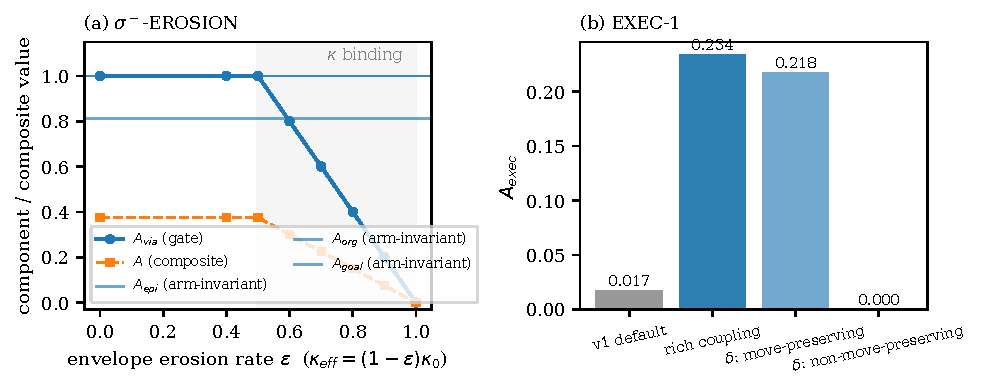
\includegraphics[width=\textwidth]{figures/fig_p3_gate_exec.pdf}
\caption{(a) $\sigma^-$-EROSION: as the capability envelope erodes
($\kappa_{eff}=(1-\varepsilon)\kappa_0$), the extended gate $\Avia$ and the
composite $A$ collapse monotonically to zero while all five channel
components and $\Lam$ stay pointwise invariant---pure viability erosion is
invisible to channel monitors and caught only by the gate (the
$n=2$ state-resource analogue is RES-1). (b) EXEC-1: the execution
channel's dynamic range, pinned near zero on the compact default instance,
is restored by richer action--observation coupling ($\Aexec=0.234$,
$13.7\times$ the v1 reading), and the $\delta$-contraction chain falls to
the exact zero-empowerment signature.}
\label{fig:p3gate}
\end{figure}

\subsection{Estimator validation (two-path discipline)}\label{sec:estimators}

Each component quantity has two implementation paths---truth (tensor
enumeration) and estimation (finite-sample from logs)---and the estimation
path is validated against the truth path on synthetic configurations
(five components; absolute errors all $\le0.0096$):

\begin{center}\small
\begin{tabularx}{\textwidth}{@{}>{\raggedright\arraybackslash}X l l l@{}}
\toprule
Quantity & Configuration & Est.\ vs truth & abs.\ err \\
\midrule
$\Aorg$ probe flow & toy + $\beta_\pi$ uniform probe arm & $0.6496\pm0.0486$
vs $0.6592$ & $0.0096$ \\
$\Avia$ ($Z$-log read) & ENV-0 baseline & $0.5248\pm0.0107$ vs $0.5344$ &
$0.0095$ \\
$\Agoal$ input $U_{eff}$ (white-box read) & ENV-0 baseline &
$1.0000\pm0.0000$ vs $1.0000$ & $<10^{-6}$ \\
$\Aepi$ input $\bar D$ (accuracy against logged truth) & ENV-0
$\gamma{=}0.5$ arm, paired seeds & $0.6573\pm0.0087$ vs $0.6587$ & $0.0014$ \\
$\Aexec^{obs}$ ($I(A_t;O_{t+1})$, passive protocol) & ENV-0 sharp-temperature
arm & $0.0103\pm0.0029$ vs $0.0104$ & $0.00009$ \\
\bottomrule
\end{tabularx}
\end{center}

\noindent Rows are five synthetic configurations; each is a single fixed
out-of-matrix run (seeds 910097--910099) with $2{,}000$--$8{,}000$ sampled
trajectories, and the $\pm$ is the trajectory-block standard error with the
Miller--Madow bias registered---not a cross-seed interval. The $\le0.0096$
bound is therefore a sampling-error statement for these configurations, not
a seed-distribution result.

\noindent Black-box rules are exercised end-to-end (BB-1): zero violations of
the certified upper end of \eqref{eq:aorg-interval} in $3/3$
bypass-semantics arms
(the reference lower end also happens to enclose the truth there; widths
$0.01/0.005/0.003$ across probe probabilities). This is a replay of the
certified direction, not an interval-containment theorem: no containment
claim is made for the lower end, and the mediation case is outside the
certificate (\S\ref{sec:blackbox}). Both protocol directions
of \S\ref{sec:blackbox} are anchored (passive observation
$\Aexec^{obs}>\Aexec$ strictly; independent probes $\le$). Two estimation
paths are explicitly \emph{not} yet instrumented and are registered as gaps,
not silently omitted: the event-level sampled carriers of $\Aref$ and $\Lam$
(endorsement-event logging), and MaxEnt-IRL black-box recovery of $\Ueff$
(white-box read used here).

\subsection{Human-side triangulation}\label{sec:triangulation}

The human-side correspondence is qualitative triangulation over published
evidence, not new subject data: self-determination theory's controlling
instruments undermine intrinsic motivation \citep{ryan_deci2000}---the
empirical counterpart of T8(i) (FORCE-1 arms); dark patterns at web scale
\citep{nouwens2020}---the $\gamma$-class manipulation of human agents whose
harms resist behavioral attribution (T2 multi-channel necessity, ATK-4); and
learned helplessness \citep{maier_seligman2016}---the signature
($\Envenv$ intact, $\EmpPi\to0$) reproduced in ATK-3(iv)/LH-1 with recovery
hysteresis. The registered validation path for the human substrate is limited
experiments plus large-scale online behavioral data under the four-phase
protocol of Section~\ref{sec:identifiability}; a minimal construct-validity
study (expert annotation of channel profiles against the composite) is the
immediate next step.

\subsection{Threats to validity}\label{sec:threats}

(i) The damage dynamics are deterministic; stochastic margin theory (unified
optimal detection $\times$ repair) and noise-induced escape versions of C1/C2
are open. (ii) The substrate is tabular; an LLM-substrate instantiation
(system prompt/memory/goal functions as $S$) is future work, and the scenario
labels are toy analogues as registered at the top of this section. (iii)
ATK-5's
time-compression curve and LH-1's recovery lag are calibrated curves, not
measured phenomena. (iv) Defense coupling is implemented for the gate/drift
classes (ATK-1/2);
coupling for ATK-3--6 is a placeholder (identical rows across defense
arms). (v) Continuous-action empowerment normalization depends on the
reference measure; cross-substrate comparisons must report it.
(vi) Sample-mode estimator intervals are block standard-error bands with
Miller--Madow bias registered, not exact confidence intervals.
(vii) The phenomenal track's per-component values are stored only as
composites, so the hallucination-index series is reported at the calibrated
weights; its weight-sensitivity is a registered gap.
(viii) The hallucination index is directional as designed: it flags
self-overestimation under covert manipulation, while self-\emph{under}estimation
(learned helplessness, where $\Aphen<A_{obj}$) leaves the $\mathrm{AHI}>0$
register silent. A minimal two-sided protocol is registered: (a) fit the
calibration map on the manipulation-free period and report both tails,
$\mathrm{AHI}^{+}=\Aphen-A_{\mathrm{obj}}$ and
$\mathrm{AHI}^{-}=A_{\mathrm{obj}}-\Aphen$; (b) use the LH-1
under-estimation arm as the positive control for the lower tail and the
ATK-2 covert arms for the upper tail; (c) report ROC/AUC and the
false-positive rate of the alarm at a pre-registered threshold. Until
(a)--(c) are run, AHI is a one-sided warning signal, never evidence.
(ix) The campaign instantiates one substrate; nothing here tests transfer to
LLM agents or humans (Section~\ref{sec:substrates}).
(x) \emph{Construct-validity sensitivity arms}: of the three arms registered
in the previous version, the two computationally cheap ones are \emph{run in
this revision} (X5 of \S\ref{sec:e2checks}; deterministic truth-mode re-runs,
artifact \texttt{analysis\_sensitivity\_arms.json}); the third remains
registered, not run. Each is stated with its protocol, its falsifier, and
its outcome.
(x-a) \emph{Endorsement-map quantization} (run): the endorsement map is
grid-quantized, and the Faith row-check (X4) exposes the plateau artifacts
this creates. The arm re-ran ATK-1 at four quantization levels---coarse
(doubled floor plateau), default, and two index-grid refinements ($k{=}2$,
$k{=}4$; utility rows linearly interpolated, a registered modeling choice
that cannot confound the goal channel, whose reading is a pure $G$-chain
functional)---across all $8$ defense configurations. \emph{Outcome}: zero
verdict flips (C1--C5 at every level); the $\dc$-normalized $\Agoal$
readings converge geometrically to the closed-form continuum-refinement
limit $\Agoal^\infty(\eta)=1-2\eta/(1+\eta)$ (stationary distance
$0.053\to0.021\to0.009$ across levels), with the default grid sitting at the
closed-form stationary gap $\eta(1-\eta)^2/\bigl(2(1+\eta)\bigr)\le0.057$
(verified pointwise); adjacent-level shifts at the campaign horizon reach
$0.036$ (partly a baseline absorption transient, gone by $T{=}8$; stationary
shift $0.032$)---beyond the SESOI of $0.01$ in absolute terms, within $5\%$
in relative terms (max $3.6\%$). The registered falsifier therefore fires on
its absolute-reading disjunct and not on its verdict disjunct; the
registered consequence stands: intermediate-strength $\Agoal$ point readings
carry a quantization band (width $\le0.057$ against the refinement limit,
closed form) rather than being point-precise, and verdict-level content is
refinement-invariant. Coarsening shifts readings by up to $0.125$: the
endorsement-grid registration obligation is non-vacuous.
(x-b) \emph{Epistemic coarse-graining $\kappa$} (run): the arm re-scored the
ATK-2 $s(\gamma)$ grid at three $\kappa$ levels---half-ring (default),
position-exact (the finest observable refinement), and the degenerate
constant $\kappa$ (boundary witness)---across all $8$ defense
configurations. \emph{Outcome}: $\Aepi$ is strictly monotone in $s(\gamma)$
at every non-degenerate level and configuration, so the registered falsifier
(non-monotone or sign-changing response under refinement) does not fire; the
level shifts baseline ($0.811\to0.778$) and deep-capture floor
($0.500\to0.250$, the random level at the finer resolution) are reported as
the sensitivity obligation of \eqref{eq:aepi} itself, and the degenerate
$\kappa$ gives $\Aepi\equiv1$ (channel uninformative by construction),
witnessing that the $\kappa$ registration cannot be dropped.
(x-c) \emph{$\Lam$ counterfactual-model choice} (registered, not run):
\eqref{eq:lambda} is a path-specific counterfactual whose value depends on
the structural model's abduction step; the registered arm recomputes $\Lam$
under two registered alternative noise models for the endorsement dynamics,
the falsifier being a sign flip of $\Lam-1$'s sign structure across models.
Until it is run, every $\Lam$ point reading carries this registration.
(xi) \emph{External substrate, pre-registered in outline}: the decisive next
experiment ports the five surgery classes to an independent substrate (a
MiniGrid-style environment with a learned tabular agent, or a simplified
LLM tool-use harness with logged internals), mirrors the proposition-level
criteria of Table~\ref{tab:main} with the same SESOI registry, and pairs
channel profiles with independent autonomy assessments for the
construct-validity half. Power: at the sample-mode estimator scale measured
here (absolute error $\le0.0096$ at $2{,}000$--$8{,}000$ trajectories,
\S\ref{sec:estimators}), detecting the registered composite SESOI of $0.01$
at two-sided $\alpha=0.05$ requires $n\approx8$ seeds for power $0.8$ under a
Gaussian noise model, so the carried-over $n=30$ seed design has power
$>0.99$; this power statement is part of the registration, not a result.

\paragraph{What would falsify the framework itself?}
The registered windows test the implementation, not the theory: a correct
replay of a definitional-layer claim cannot disconfirm it. The framework's
substantive falsifier is external. If, across substrates, the five-channel
profile fails to predict independent autonomy assessments---or if a coarser
account (fewer channels, a single scalar, or a plain behavioral audit)
predicts them as well or better---then the channel choice is disconfirmed,
however well the algebra behaves. Within the substrate, this revision's
checks already speak to the coarser-account disjunct: the scalar functional
baseline $\bar u$ dissociates from $A$ in two of three regimes, and freezing
any single channel destroys unique attack attribution in at least one
campaign (\S\ref{sec:e2checks}). The cross-substrate disjunct is unaffected
by these checks: external-substrate validation remains the decisive next
experiment rather than a formality
(Section~\ref{sec:limitations}).
